% ============================================================================
% CHAPTER 5: WBS
% ============================================================================

\chapter[Work Breakdown Structure]{Work Breakdown Structure (WBS)}

\vspace{12pt}

% ============================================================================
\section{WBS Overview}

\par The Work Breakdown Structure organizes project deliverables and work into smaller, more manageable components. Each level provides increasing detail about the work required to complete the project successfully.





\section{WBS Visual Representation}

\begin{figure}[H]
    \centering
    % WBS diagram created in MS Visio
    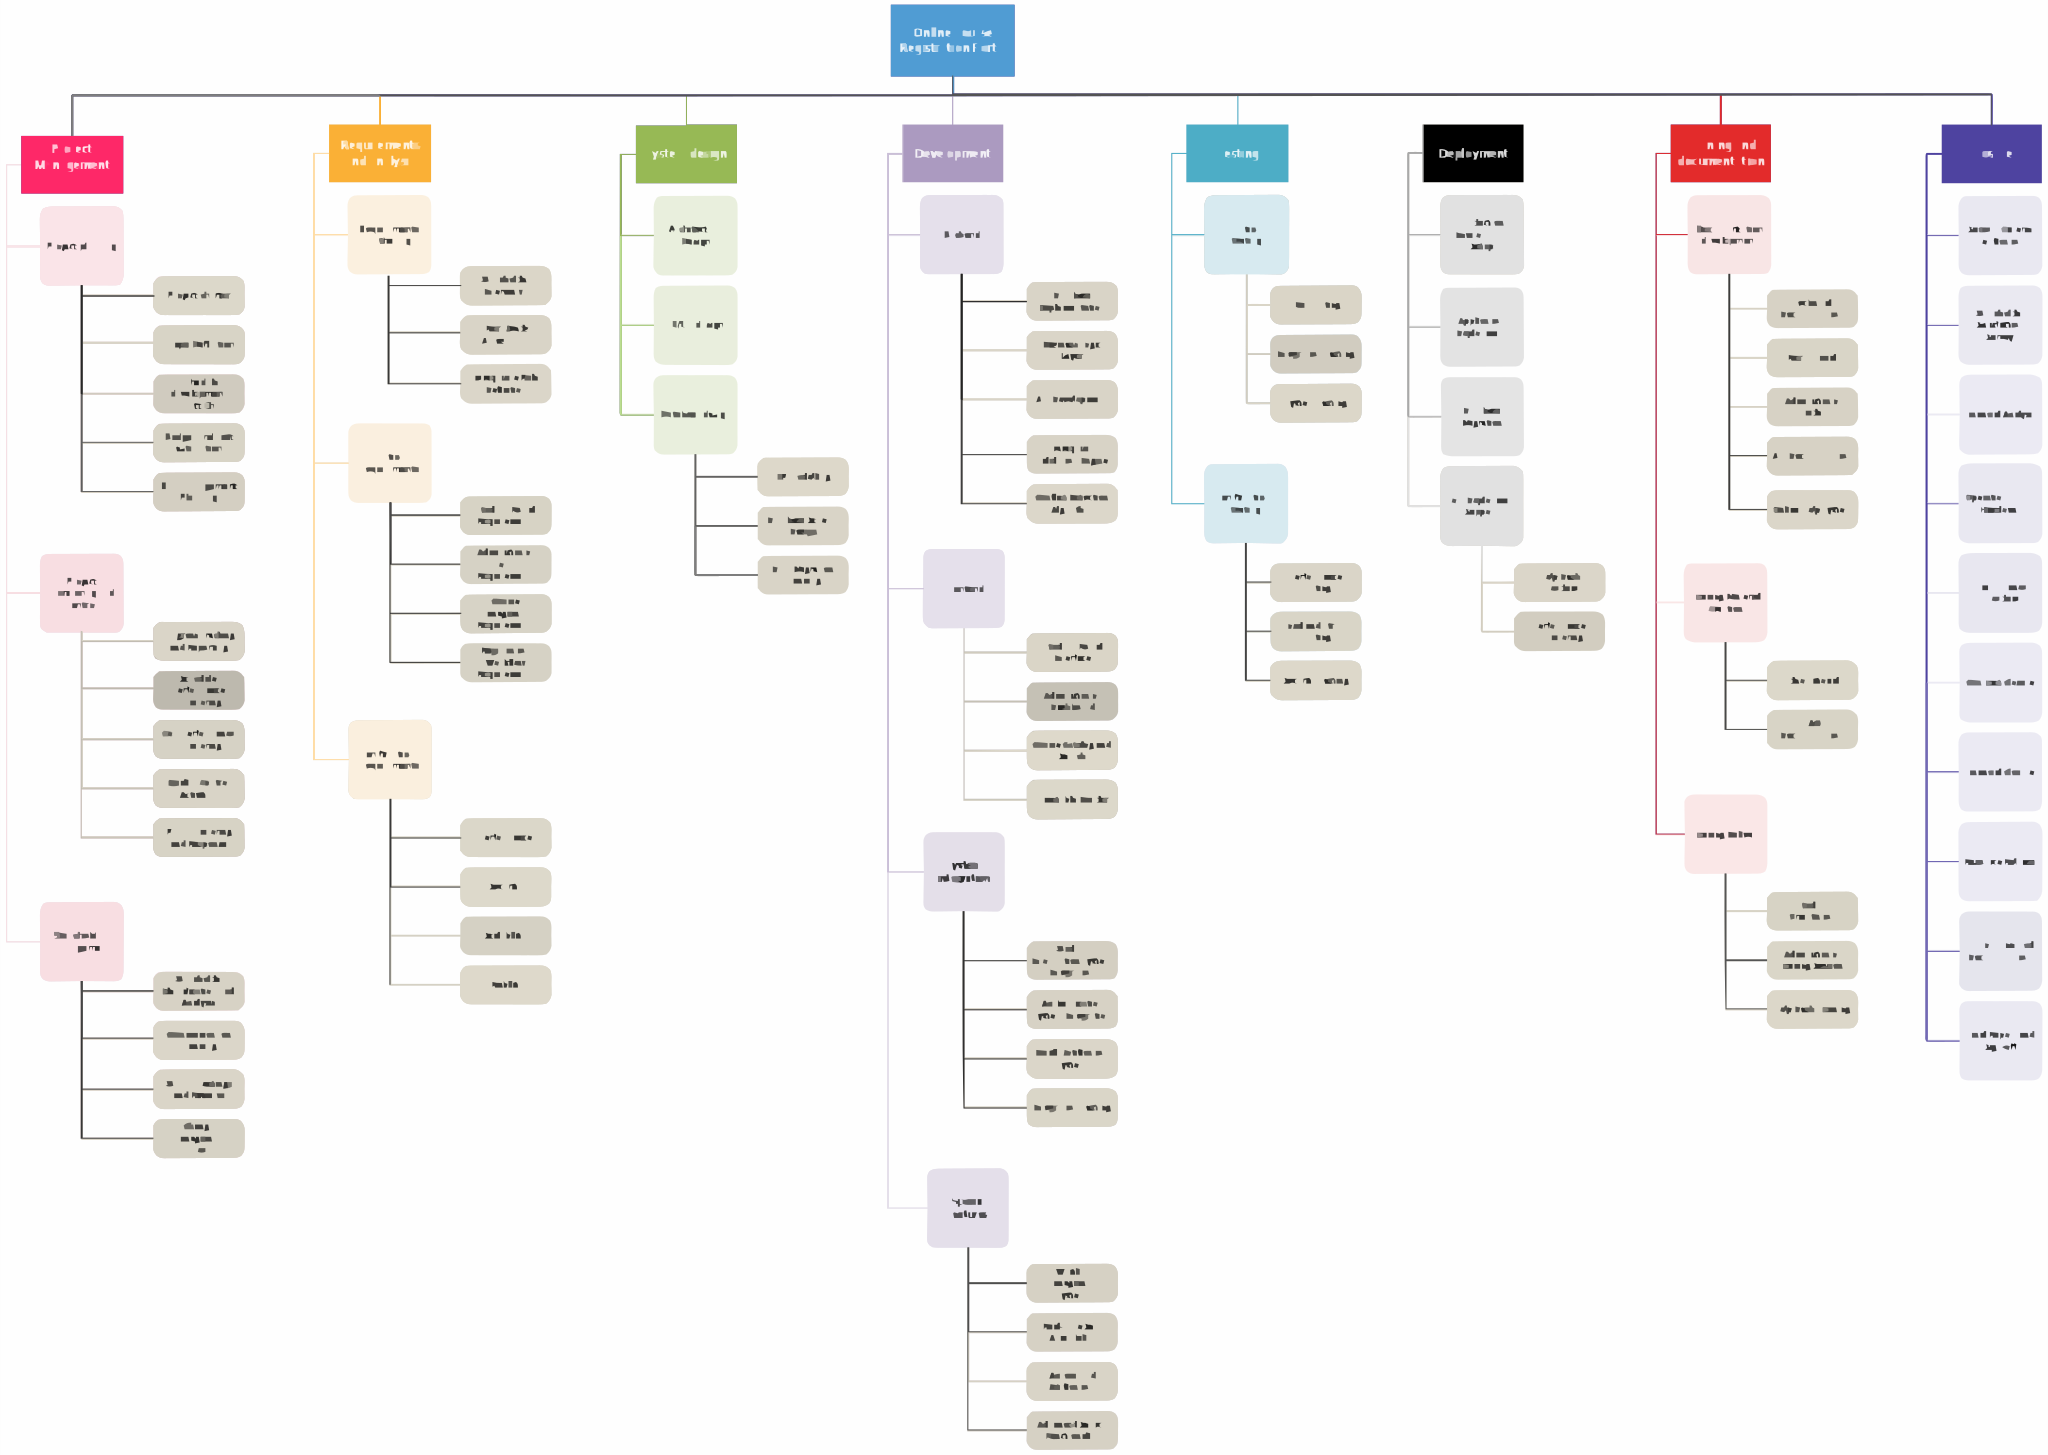
\includegraphics[width=\textwidth]{images/wbs.pdf}
    \caption{Work Breakdown Structure - Visual Hierarchy}
    \label{fig:wbs-diagram}
\end{figure}

% ============================================================================
\section{WBS Dictionary Sample}

\par The following table provides a sample of WBS dictionary entries for selected work packages:

\begin{table}[H]
\centering
\caption{WBS Dictionary Sample Entries}
\begin{tabularx}{\textwidth}{|l|X|}
\hline
\textbf{WBS Code} & 1.4.1.4 \\
\hline
\textbf{Name} & Prerequisite Validation Engine \\
\hline
\textbf{Description} & Develop the core engine that validates student prerequisite requirements before allowing course registration \\
\hline
\textbf{Responsible} & Backend Development Team \\
\hline
\textbf{Duration} & 2 weeks \\
\hline
\textbf{Resources} & 2 Senior Developers, 1 QA Engineer \\
\hline
\textbf{Dependencies} & Prerequisite rules definition (1.2.1.3), Database implementation (1.4.1.1) \\
\hline
\textbf{Deliverables} & Functional prerequisite validation module, unit tests, documentation \\
\hline
\end{tabularx}
\end{table}

% ============================================================================


